\section{Marktvormen}

Wat is een \entry{marktvorm}? Het is een wijze van ontmoeting tussen vragers en aanbieders. We onderscheiden een aantal type marktvormen op basis van het aantal aanbieders en op basis van de differentiatie van de verkochte producten (zie tabel \ref{tab:h3vormen}). De meest gekende zijn volmaakte mededinging en het monopolie. Beide zijn eerder theoretisch en dienen als toetssteen.

\begin{table}[H]
\small\centering\captionsetup{justification=centering,margin=2cm}
\begin{tabular}{c | c | c | c}
\textbf{Aantal aanbieders} $\rightarrow$ & \textbf{1} & \textbf{Enkele} & \textbf{Veel}\\
\textbf{Differentiatie} $\downarrow$ & & & \\
\hline
\textbf{Homogeen} & Monopolie & Homogeen oligopolie & Volmaakte mededinging \\
\textbf{Heterogeen} & & Heterogeen oligopolie & Monopolistische mededinging \\
\end{tabular}
\caption{Type marktvormen (\entrystyled{homogeen}{homogene} producten zijn in de ogen van de afnemer steeds hetzelfde - kwaliteit, merk en service maken bijvoorbeeld niet uit)}
\label{tab:h3vormen}
\end{table}

We gaan hier nu dieper op in. Merk wel op! \textit{We gaan ervan uit dat er veel consumenten (vragers) zijn, dat alle marktpartners perfect ge\"informeerd zijn, en dat ze zich optimaal gedragen} (zie \ref{sec:h0oea}). 
\par We focussen eigenlijk op \'e\'en probleem ; het kiezen van de hoeveelheden zodanig dat het verschil tussen totale `opbrengst' en totale `kost' ($TW(q)=TO(q)-TK(q)$) zo groot mogelijk wordt.  Wat overeenkomt met het gelijkstellen van de marginale opbrengst aan de marginale kost.
\par Voor de producent is de opbrengst gelijk aan de ontvangst (de marginale opbrengst is de ontvangst voor de laatst verkochte eenheid), en is de kost alles wat nodig is om te produceren (dit gaat niet altijd over geld).
\par Voor de consument is de opbrengst gelijk aan zijn subjectieve waardering (de marginale opbrengst is de marginale betalingsbereidheid). De kost is wat hij moet betalen.\\

\par Ons oogpunt is \entrystyled{normatieve uitspraak}{normatief} ; wij gaan de marktvormen vergelijken door gebruik te maken van het begrip \entrystyled{pareto-efficientie}{Pareto-effici\"entie}\footnote{Vilfredo Pareto was een Italiaans econoom die vroegtijdig aanhanger was van het liberalisme, maar zich later bekeerde tot het fascisme.}. Een \entrystyled{pareto-verbetering}{Pareto-verbetering}\footnote{Het begrip Pareto-effici\"entie hangt samen met de \entry{productiemogelijkhedencurve} (hoofdstuk \ref{sec:h1comp}) ; punten op de curve stellen Pareto-effici\"ente situaties voor. Gaat men van een punt \textit{binnen} de curve naar een punt \textit{op} de curve, dan heeft men te maken met een Pareto-verbetering.} betekent in deze context dat \'e\'en marktpartner erop vooruit gaat zonder dat een andere partner erop achteruit gaat. Een stituatie is dan Pareto-effici\"ent als men onmogelijk de welvaart van \'e\'en iemand kan verhogen zonder die van een andere te verlagen.
\par Aan de \textit{verdeling} van de welvaart hechten we \textit{geen enkel} belang (dat komt later aan bod)!

\begin{figure}[H]
\vspace{0.5cm}
\centering
\captionsetup{justification=centering,margin=2cm}
\begin{tikzpicture}
	\begin{axis}[name=left,xlabel={Welvaart Lisa}, ylabel={Welvaart Bart}, ymin=0,ymax=120,xmin=0,xmax=120,width=5cm, height=5cm]
		\addplot[gray, samples=100, domain=0:100]{100-(x*x)/100};
		\draw[fill=black] (20,96) circle (2) node[above right] {A};
		\draw[fill=black] (60,64) circle (2) node[above right] {B};
		\draw[fill=black] (90,19) circle (2) node[above right] {C};
       		\draw[fill=black] (40,40) circle (2) node[left] {D};
		\addplot+[draw=none,mark=none,pattern=flexible hatch, samples=100, domain=0:100, area legend, pattern color=gray!20]{100-(x*x)/100} \closedcycle;
	\end{axis}
\end{tikzpicture}
\caption{Een aantal situaties : A, B en C zijn Pareto-effici\"ent en D is Pareto-ineffici\"ent}
\label{fig:h3peff}
\end{figure}

\subsection{Volmaakte Mededinging}

\subsubsection{De Vraag Vereenvoudigd}\label{sec:vraageenvoudig}

\entrystyled{volmaakte mededinging}{Volmaakte mededinging} is een marktvorm gekenmerkt door vele aanbieders van homogene producten. Bij diens beschouwing vereenvoudigen we de vraag ; we veronderstellen dat de marginale betalingsbereidheid van de consument daalt met de geconsumeerde hoeveelheid, en dat hij \entrystyled{prijsnemerschap}{prijsnemer} is. Hij zal consumeren tot zijn marginale betalingsbereidheid gelijk is aan de prijs van het product ($MO=MBB=P=MK$).\\

\par Een mogelijke vraagcurve van \'e\'en individu wordt gegeven in figuur \ref{fig:h3vraag}(a). Om van dergelijke individuele vraagcurven over te gaan naar de marktvraag moet men de afzonderlijke curven \textit{horizontaal} optellen (figuur \ref{fig:h3vraag}(b)).

\begin{figure}[H]
\centering
\captionsetup{justification=centering,margin=2cm}
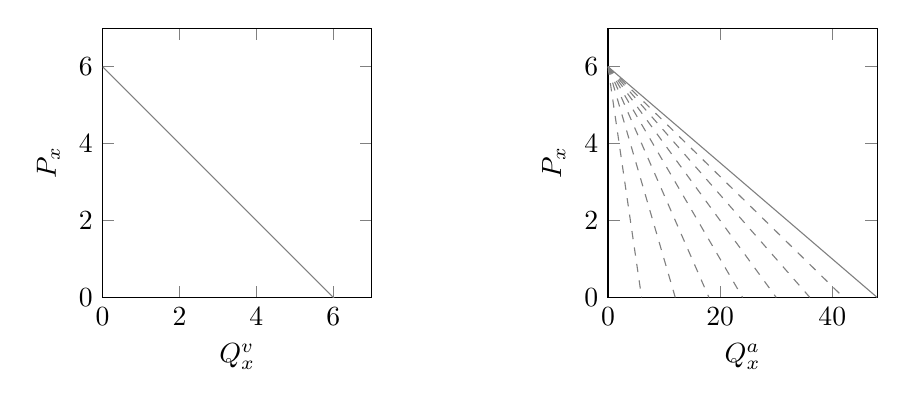
\begin{tikzpicture}
	\begin{axis}[name=left,xlabel=$Q_x^v$, ylabel=$P_x$, ymin=0, xmin=0, xmax=7, ymax=7,width=5cm, height=5cm]
		\addplot[gray, samples=50, domain=0:7] {6-x};
	\end{axis}
	\begin{axis}[xshift=3cm,at={(left.north east)},anchor=north west,xlabel=$Q_x^a$, ylabel=$P_x$, ymin=0, xmin=0, xmax=48, ymax=7,width=5cm, height=5cm]
		\addplot[gray, dashed, samples=120, domain=0:6] {6-x};
		\addplot[gray, dashed, samples=120, domain=0:12] {6-0.5*x};
		\addplot[gray, dashed, samples=120, domain=0:18] {6-(1/3)*x};
		\addplot[gray, dashed, samples=120, domain=0:24] {6-(1/4)*x};
		\addplot[gray, dashed, samples=120, domain=0:30] {6-(1/5)*x};
		\addplot[gray, dashed, samples=120, domain=0:36] {6-(1/6)*x};
		\addplot[gray, dashed, samples=120, domain=0:42] {6-(1/7)*x};
		\addplot[gray, samples=50, domain=0:48] {6-(1/8)*x};
	\end{axis}
\end{tikzpicture}
\caption{(a) Individuele marktvraag, \\(b) Overschakeling naar marktvraag (hier gaat het over identieke consumenten)}
\label{fig:h3vraag}
\end{figure}

\subsubsection{Het Aanbod}

Het aanbod is wat ingewikkelder. We kijken eerst naar de \entry{schaalopbrengsten}. Wat zijn schaalopbrengsten? Als we de productiefactoren (zowel arbeid als kapitaal) doen stijgen met $x$ procent, en de productie daardoor verhoogt met $y$ procent, dan zijn de schaalopbrengsten :
\begin{itemize}
\item[-] \textit{stijgend} als $y>x$ (men heeft het over \term{schaalvoordelen}). De productie stijgt dus sneller dan de productiefactoren en de gemiddelde kost daalt. Dit kan te wijten zijn aan ondeelbaarheden (je kan geen halve computer kopen, maar de eerste computer die je koopt zal je waarschijnlijk ook kunnen inzetten als er nieuwe klanten bijkomen) en specialisatie.
\item[-] \textit{dalend} als $y<x$ (men heeft het over \term{schaalnadelen}). De productie stijgt minder snel dan de productiefactoren en de gemiddelde kost stijgt. Dit kan te wijten zijn aan technische begrenzingen (eg. computer kan niet m\'e\'er aan), omgevingsfactoren (eg. ruimte ontbreekt) of organisatorische problemen (grotere bedrijven zijn moeilijker te beheren).
\item[-] \textit{constant} als $y=x$. De productie stijgt even snel als de productiefactoren en de gemiddelde kost is constant.
\end{itemize}
Bedrijven gaan dan ook fusioneren als er daar schaalvoordelen bij komen kijken, en splitsen als er schaalnadelen zijn en het bedrijf te groot wordt.\\

\par De schaalopbrengsten zijn dus af te lezen uit (gemiddelde) kostenfuncties. Stel, de functie van de totale kost is $TK=0,025q^3-0,6q^2+18,6q$. De gemiddelde kost (de totale kost gedeeld door de hoeveelheid) is dan $GK=0,025q^2-0,6q+18,6$ en de marginale kost (zie hoofdstuk \ref{sec:appafg}) is $MK=0,075q^2-1,2q+18,6$. Deze functies zijn uitgezet in figuur \ref{fig:h3aanbod}.

\begin{figure}[H]
\vspace{0.5cm}
\centering
\captionsetup{justification=centering,margin=2cm}
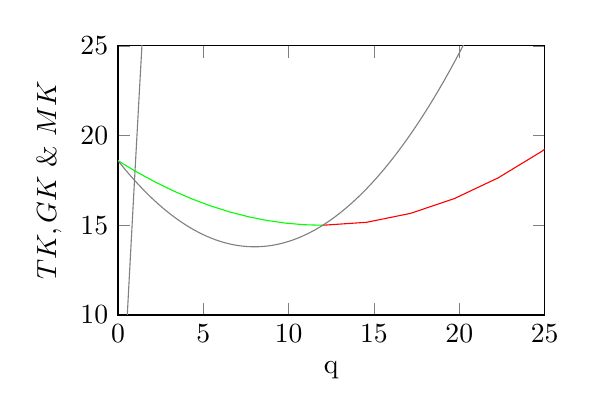
\begin{tikzpicture}
	\begin{axis}[name=left,xlabel={q}, ylabel={$TK,GK\ \&\ MK$}, ymin=10,ymax=25,xmin=0,xmax=25,width=7cm, height=5cm]
		\addplot[gray, samples=100, domain=0:30]{0.025*x^3-0.6*x^2+18.6*x};
		\addplot[green, samples=12, domain=0:12]{0.025*x^2-0.6*x+18.6};
		\addplot[red, samples=8, domain=12:30]{0.025*x^2-0.6*x+18.6};
		\addplot[gray, samples=100, domain=0:30]{0.075*x^2-1.2*x+18.6};
	\end{axis}
\end{tikzpicture}
\caption{Kostenfuncties in volmaakte mededinging (de gemiddelde kost daalt zolang de marginale kost eronder ligt, en omgekeerd)}
\label{fig:h3aanbod}
\end{figure}

Voor de marginale \textit{opbrengst} gaan we uit van prijsnemerschap : de individuele producent is prijsnemer, de gemiddelde opbrengst (prijs) is gelijk aan de marginale opbrengst. We nemen in ons voorbeeld als prijs $P=17$ (figuur \ref{fig:h3aanbod2}).

\begin{figure}[H]
\vspace{0.5cm}
\centering
\captionsetup{justification=centering,margin=2cm}
\begin{tikzpicture}
	\begin{axis}[name=left,xlabel={q}, ylabel={$GO=MO,GK\ \&\ MK$}, ymin=12,ymax=21,xmin=0,xmax=25,width=5cm, height=5cm]
		\addplot[gray, samples=100, domain=0:25]{17};
		\addplot[green, samples=12, domain=0:12]{0.025*x^2-0.6*x+18.6};
		\addplot[red, samples=8, domain=12:25]{0.025*x^2-0.6*x+18.6};
		\addplot[gray, samples=100, domain=0:25]{0.075*x^2-1.2*x+18.6};
		\addplot[gray, dashed] coordinates {(14.5,0) (14.5,15.16)};
		\addplot[blue] coordinates {(14.5,15.16) (14.5,17)};
		\addplot[draw=none,pattern=north west lines, pattern color=gray!20] coordinates {(0,15.16) (14.5,15.16) (14.5,17) (0,17)};
	\end{axis}
\end{tikzpicture}
\caption{Kosten en opbrengst van de producent in volmaakte mededinging}
\label{fig:h3aanbod2}
\end{figure}

Merk op dat er in de figuur \textit{twee} punten zijn waar $MK=MO$. In het eerste punt is de gemiddelde kost echter groter dan de gemiddelde opbrengst. De producent maakt verlies! Het is dus in het tweede punt dat de hoeveelheid bepaald wordt, de producent zal $q=14.53$ (verticale stippellijn) produceren. Bij deze hoeveelheid is het verschil tussen de prijs en de gemiddelde kost gelijk aan de \textit{gemiddelde winst} $GW$ (blauwe verticale lijn).
\par De producent wilt niet de gemiddelde winst maar de \textit{totale winst} maximaliseren. Dit is gelijk aan de hoeveelheid $q$ vermenigvuldigd met de gemiddelde winst (gearceerd gebied).\\

\par Stel nu dat we niet uitgaan van een prijs $P=17$. Dan kan je inzien dat de aangeboden hoeveelheid steeds overeenkomt met het punt op de marginale kostenfunctie waar $MO=P=MK$. Het zijn dus alle punten op deze curve waar $MK>=GK$ (of waar $TO>=TK$) die de aanbodfunctie voorstellen (zie figuur \ref{fig:h3aanbod3})!

\begin{figure}[H]
\vspace{0.5cm}
\centering
\captionsetup{justification=centering,margin=2cm}
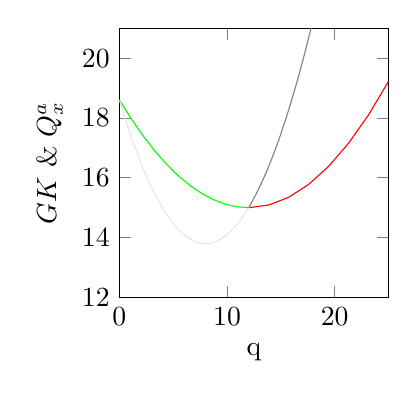
\begin{tikzpicture}
	\begin{axis}[name=left,xlabel={q}, ylabel={$GK$ \& $Q_x^a$}, ymin=12,ymax=21,xmin=0,xmax=25,width=5cm, height=5cm]
		\addplot[green, samples=12, domain=0:12]{0.025*x^2-0.6*x+18.6};
		\addplot[red, samples=8, domain=12:25]{0.025*x^2-0.6*x+18.6};
		\addplot[gray, samples=50, domain=12:25]{0.075*x^2-1.2*x+18.6};
		\addplot[gray!20, samples=50, domain=0:12]{0.075*x^2-1.2*x+18.6};
	\end{axis}
\end{tikzpicture}
\caption{Aanbodfunctie in volmaakte mededinging}
\label{fig:h3aanbod3}
\end{figure}

Deze aanbodfunctie is die van juist \'e\'en producent. Om over te schakelen naar het marktaanbod moet men de individuele aanbiedingen \textit{horizontaal} optellen. 
\par Het is echter z\'o dat het aantal ondernemingen in volmaakte mededinging veranderlijk is. Er is \term{vrije toetreding} ; als er winst wordt gemaakt komen er bedrijven bij, als er verlies is, is er uittreding (dat laatste noemt men \entry{creatieve destructie}).
\par Een evenwicht (van de industrie) wordt bereikt als er geen toe- en uittreding van bedrijven meer is. De bedrijven willen altijd dat $P=MK$. Door vrije toe- en uittreding is het ook zo dat $P=GK$ (de winst verdwijnt\footnote{Als bedrijven toetreden op de markt gaat de marktaanbodcurve naar rechts verschuiven en vlakker worden, en zal er een aanbodoverschot zijn. Daardoor verlaagt de prijs. Dit gaat door zolang er in de sector winst is, gezien er vrije toetreding is en bedrijven uit zijn op winst.}). En dus is de prijs $P$ gelijk aan de minimale gemiddelde kost $GK$. De prijs is \term{endogeen} bepaald.
\par De vraag heeft geen invloed op de prijs, maar wel op het aantal bedrijven.\\

\par In dit systeem is de consument de grote winnaar, want er wordt geproduceerd tegen de laagst mogelijke gemiddelde kost. En de winst? Die is verdwenen. Maar dat is geen probleem ; de producent wordt nog steeds vergoed voor zijn moeite (eigen arbeid en vermogen wordt in rekening gebracht in de totale kost).

\subsubsection{Welvaartsanalyse}

Figuur \ref{fig:h3vmew} stelt een marktevenwicht bij volmaakte mededinging voor. Het aanbod is perfect elastisch. Het gearceerde gebied is het consumentensurplus.
\par Gezien dit surplus maximaal is, heeft men te maken met \entrystyled{pareto-efficientie}{Pareto-effici\"entie}.

\begin{figure}[H]
\vspace{0.5cm}
\centering
\captionsetup{justification=centering,margin=2cm}
\begin{tikzpicture}
	\begin{axis}[name=left,xlabel={q}, ylabel={$P$}, ymin=0,ymax=7,xmin=0,xmax=600,width=5cm, height=5cm]
		\addplot[blue, samples=50, domain=0:600]{6-(1/100)*x};
		\addplot[red, samples=50, domain=0:
		600]{2};
		\addplot[draw=none,pattern=north west lines, pattern color=gray!30] coordinates {(0,2) (400,2) (0,6)};
	\end{axis}
\end{tikzpicture}
\caption{Marktevenwicht in volmaakte mededinging}
\label{fig:h3vmew}
\end{figure}

Een belasting op de producent zal de aanbodcurve naar boven doen schuiven en het consumentensurplus verkleinen.
\par Er is dus een welvaartsverlies (figuur \ref{fig:h3vmewb}, gearceerd).

\begin{figure}[H]
\vspace{0.5cm}
\centering
\captionsetup{justification=centering,margin=2cm}
\begin{tikzpicture}
	\begin{axis}[name=left,xlabel={q}, ylabel={$P$}, ymin=0,ymax=7,xmin=0,xmax=600,width=5cm, height=5cm]
		\addplot[blue, samples=50, domain=0:600]{6-(1/100)*x};
		\addplot[red, samples=50, domain=0:
		600]{2};
		\addplot[draw=none,pattern=north west lines, pattern color=gray!50] coordinates {(300,2) (300,3) (400,2)};
		\addplot[red!40, samples=50, domain=0:
		600]{3};
	\end{axis}
\end{tikzpicture}
\caption{Marktevenwicht in volmaakte mededinging - met belasting op de producent}
\label{fig:h3vmewb}
\end{figure}

Een bindende minimumprijs heeft een gelijkaardig effect. \\

\par Als de overheid subsidieert, dan vergroot het consumentensurplus. Dat is echter geen goede zaak, want de overheid betaalt meer dan dat surplus. Er is een netto welvaartsverlies (figuur \ref{fig:h3vmews}, gearceerd).

\begin{figure}[H]
\vspace{0.5cm}
\centering
\captionsetup{justification=centering,margin=2cm}
\begin{tikzpicture}
	\begin{axis}[name=left,xlabel={q}, ylabel={$P$}, ymin=0,ymax=7,xmin=0,xmax=600,width=5cm, height=5cm]
		\addplot[blue, samples=50, domain=0:600]{6-(1/100)*x};
		\addplot[red, samples=50, domain=0:
		600]{2};
		\addplot[draw=none,pattern=north west lines, pattern color=gray!50] coordinates {(400,2) (500,2) (500,1)};
		\addplot[blue!40, samples=50, domain=0:
		600]{1};
	\end{axis}
\end{tikzpicture}
\caption{Marktevenwicht in volmaakte mededinging - met subsidie van de producent}
\label{fig:h3vmews}
\end{figure}

\subsection{Monopolie}

\subsubsection{Definitie}

Het \entry{monopolie} is een theoretische tegenpool van de volmaakte mededinging. Het is een marktvorm met juist \'e\'en aanbieder van een  product zonder goede substituten. Deze aanbieder heeft daardoor een machtspositie. Hij kan zich als \term{prijszetter} gedragen, want door zijn te produceren hoeveelheid aan te passen verandert hij meteen de prijs van zijn product.
\par Deze machtspositie is echter relatief ; de keuzes van de monopolist worden beperkt door de marktvraagcurve. Hij moet kiezen tussen kleine verkoop bij grote prijzen of grote verkoop bij lage prijzen. Zoals gewoonlijk wil hij, om zijn winst te maximaliseren, dat de marginale opbrengst gelijk is aan de marginale kost.\\

\subsubsection{Winstmaximalisatie bij Monopolie}

We nemen als voorbeeld een eenvoudige vraagfunctie, $q_x^v=10-p_x$. De prijs (gemiddelde ontvangst) is dan $p=10-q$. De totale ontvangst is $TO=p\cdot q=10q-q^2$. De marginale ontvangst is hier de afgeleide van, $MO=10-2q$ (zie hoofdstuk \ref{sec:appafg}).\par Merk op dat de marginale opbrengst kleiner is dan de gemiddelde opbrengst, de prijs. De monopolist moet concessies doen. Verkoopt hij meer producten, dan moet dit aan een lagere prijs (hij moet voor iedereen dezelfde prijs vragen).\\

\par Laten we nu vertrekken van de vraagfunctie $q_x^v=600-100p_x$. De prijs (gemiddelde opbrengst) is $p=6-\frac{1}{100}q=6-0.01q$, de totale opbrengst $TO=6q-0.01q^2$ en de marginale opbrengst $MO=6-0.02q$ (figuur \ref{fig:h3opmonop}).

\begin{figure}[H]
\vspace{0.5cm}
\centering
\captionsetup{justification=centering,margin=2cm}
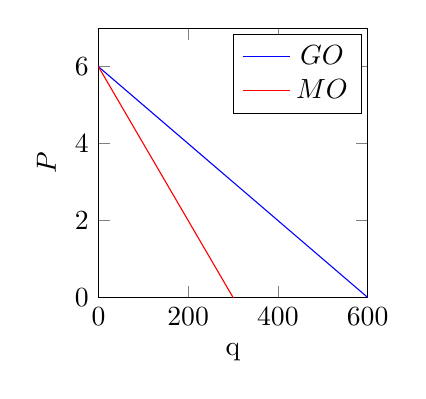
\begin{tikzpicture}
	\begin{axis}[name=left,xlabel={q}, ylabel={$P$}, ymin=0,ymax=7,xmin=0,xmax=600,width=5cm, height=5cm]
		\addplot[blue, samples=50, domain=0:600]{6-(1/100)*x};
		\addplot[red,samples=50, domain=0:600]{6-(2/100)*x};
		\legend{$GO$,$MO$}
	\end{axis}
\end{tikzpicture}
\caption{Gemiddelde en marginale opbrengst bij monopolie}
\label{fig:h3opmonop}
\end{figure}

Bij het monopolie is er geen aanbodcurve. De monopolist produceert een hoeveelheid, bijvoorbeeld $q=200$. In dat geval zal hij zijn prijs zetten op 4 euro, want dan is zijn producentensurplus het grootst (figuur \ref{fig:h3opmonop}(a)). Het consumentensurplus (figuur \ref{fig:h3opmonop}(b)) is kleiner dan in volmaakte mededinging.
\par Gezien de consumenten meer verliezen dan dat de producent winnen, is er een welvaartsverlies. Hoe lost men dat op?

\begin{figure}[H]
\centering
\captionsetup{justification=centering,margin=2cm}
\begin{tikzpicture}
	\begin{axis}[name=left,xlabel={q}, ylabel={$P$}, ymin=0,ymax=7,xmin=0,xmax=600,width=5cm, height=5cm]
		\addplot[blue, samples=50, domain=0:600]{6-(1/100)*x};
		\addplot[red,samples=50, domain=0:600]{6-(2/100)*x};
		\addplot[draw=none,pattern=north west lines, pattern color=gray!50] coordinates {(0,2) (0,4) (200,4) (200,2)};
		\legend{$GO$,$MO$}
	\end{axis}
	\begin{axis}[xshift=3cm,at={(left.north east)},anchor=north west,xlabel={q}, ylabel={$P$}, ymin=0,ymax=7,xmin=0,xmax=600,width=5cm, height=5cm]
		\addplot[blue, samples=50, domain=0:600]{6-(1/100)*x};
		\addplot[red,samples=50, domain=0:600]{6-(2/100)*x};
		\addplot[draw=none,pattern=north west lines, pattern color=gray!50] coordinates {(0,6) (0,4) (200,4)};
		\legend{$GO$,$MO$}
	\end{axis}
\end{tikzpicture}
\caption{(a) Het producentensurplus bij monopolie, \\(b) Het consumentensurplus bij monopolie}
\label{fig:h3opmonop2}
\end{figure}

\subsubsection{Prijsdiscriminatie}

Laten we er even van uit gaan dat de monopolist perfect ge\"informeerd is (hij weet iedereens betalingsbereidheid), en dat hij kan verhinderen dat zijn klanten onder elkaar doorverkopen. Dan is \entry{perfecte prijsdiscriminatie} mogelijk. Hij kan voor elke klant een verschillende prijs vragen voor zijn product. Wat is nu de prijs? Die wordt de marginale ontvangst. Er is niet \'e\'en, maar oneindig veel prijzen. De marginale kost en ontvangst zijn gegeven in figuur \ref{fig:h3opmonop3}.

\begin{figure}[H]
\vspace{0.5cm}
\centering
\captionsetup{justification=centering,margin=2cm}
\begin{tikzpicture}
	\begin{axis}[name=left,xlabel={q}, ylabel={$P$}, ymin=0,ymax=7,xmin=0,xmax=600,width=5cm, height=5cm]
		\addplot[blue, samples=50, domain=0:600]{6-(1/100)*x};
		\addplot[gray,samples=50, domain=0:600]{2};
		\addplot[draw=none,pattern=north west lines, pattern color=gray!50] coordinates {(0,2) (0,6) (400,2)};
		\legend{$MO$,$MK$}
	\end{axis}
\end{tikzpicture}
\caption{Marginale ontvangst en kost bij perfecte prijsdiscriminatie (het producentensurplus is gearceerd)}
\label{fig:h3opmonop3}
\end{figure}

De evenwichtshoeveelheid wordt hier $q=400$, want daar is $MO=MK$. Het producentensurplus (gearceerd) is hier maximaal, het consumentensurplus is nul.
\par Het monopolie met perfecte prijsdiscriminatie is dus \entrystyled{pareto-efficientie}{Pareto-effici\"ent}.\\

\par Prijsdiscriminatie kan ook via \entry{marktsegmentatie}. Dat betekent dat de monopolist de markt zal opdelen in groepen. Per leeftijd, bijvoorbeeld. Zoals bij de bioscoop, waar jongeren minder betalen dan volwassenen\footnote{De bioscoop zal doen alsof dat `uit liefde voor de jeugd' wordt gedaan. De realiteit is dat het bedrijf gewoon meer wint. De jongeren hebben immers een kleiner budget, en wie een kleiner budget heeft kijkt meer naar de prijs.}.\\

\par Daarnaast kan prijsdiscriminatie ook via \term{zelfselectie}. Doorheen de tijd, bijvoorbeeld. Tijdens de vakantie of tijdens het weekend zal het huren van een appartement duurder zijn. Of men rekent eerst hoge prijzen aan, daarna lagere (bij solden). De drempel is hier dat de klant het risico loop dat de voorraad is uitgeput.
\par Men kan ook prijsverschillen hanteren die buiten proportie zijn met de kosten-verschillen. Bij Starbucks zullen cappuccino's veel meer kosten dan gewone koffies, want de klanten die dat kopen zijn bereid veel meer te betalen. Bij de verkoop van \textit{fair trade} koffie kan je hier ook mee te maken hebben.
\par Ten slotte kan prijsdiscriminatie ook bij internetaankopen ; men discrimineert bijvoorbeeld op basis van de gebruikte laptop. Gebruikers van \textit{Apple} computers zullen waarschijnlijk bereid zijn meer te betalen ...

\subsubsection{Het Natuurlijk Monopolie}

Het \entry{natuurlijk monopolie} wordt gekenmerkt door toenemende \entry{schaalopbrengsten} (schaalvoordelen). Hoe groter het bedrijf, hoe beter. Als dit geldt, dan zal er maar \'e\'en bedrijf overblijven.\\

\par Schaalvoordelen kan men categoriseren :
\begin{itemize}
\item[-] \term{statische schaalvoordelen} : als grotere ondernemingen lagere gemiddelde kosten hebben dan kleinere ondernemingen (de gemiddelde kostencurve daalt).
\item[-] \term{dynamische schaalvoordelen} : als oudere ondernemingen lagere gemiddelde kosten hebben dan debuterende. Hier speelt \textit{`learning by doing'} een rol ; een startend bedrijf maakt fouten, en doet er dan steeds minder.
\item[-] \term{netwerkexternaliteiten} : als meer consumenten kiezen voor hetzelfde product en bedrijven daardoor positieve effecten ondervinden. Zoals bij \textit{facebook} ; hoe meer mensen de website gebruiken, hoe interessanter ie wordt.
\end{itemize}
Dynamische schaalvoordelen zijn slecht voor ontwikkelingslanden, omdat ze het dan moeilijk gaan hebben om te industrialiseren. Protectie (weerhouden van import) kan dan nuttig zijn, want dit beschermt de eigen markt tegen goedkope import\footnote{Dit argument voor protectie noemt men de \term{infant industry argument}.}.\\

\par Als een bedrijf toenemende schaalopbrengsten (schaalvoordelen) heeft, dan ontstaat op natuurlijke wijze een monopolie. Er is plaats voor maar \'e\'en bedrijf.

\begin{figure}[H]
\vspace{0.5cm}
\centering
\captionsetup{justification=centering,margin=2cm}
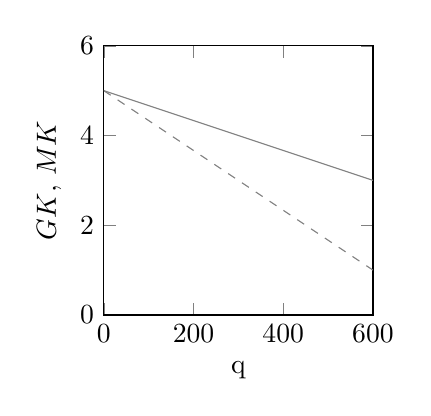
\begin{tikzpicture}
	\begin{axis}[name=left,xlabel={q}, ylabel={$GK$, $MK$}, ymin=0,ymax=6,xmin=0,xmax=600,width=5cm, height=5cm]
		\addplot[gray, samples=50, domain=0:600]{5-(1/300)*x};
		\addplot[gray,dashed,samples=50, domain=0:600]{5-(1/150)*x};
	\end{axis}
\end{tikzpicture}
\caption{Kostenverloop bij een natuurlijk monopolie}
\label{fig:h3natmon}
\end{figure}

Figuur \ref{fig:h3natmon} geeft een voorbeeld van statische schaalvoordelen van netwerkindustrie\"en. Het komt voor bij \entrystyled{nutsbedrijf}{nutsbedrijven}.

\subsubsection{Welvaartsanalyse}

We zagen eerder al dat een monopolie zonder prijsdiscriminatie gepaard gaat met welvaartsverlies. Dit is niet het geval bij perfecte prijsdiscriminatie.\\

\par Welvaartsverlies bij het monopolie bestrijdt je \textit{niet} met belastingen. Stel, men belast de monopolist met 50\%. Dan gaat de monopolist zijn gedrag niet veranderen, want wat hij moet doen om zijn winst te maximaliseren blijft hetzelfde.
\par Hoewel belastingen dus marktconform zijn, zijn ze niet aangewezen.\\

\par Nee, men doet eerder aan \entry{marginal cost pricing} : men legt een \entry{bindende maximumprijs} op die spoort met de marginale kost. Dit is echter moeilijk toe te passen, omdat de overheid de marginale kost niet kent. In het beste geval zal de monopolist liegen. In het slechtste geval zal hij de kosten artificieel opdrijven door bijvoorbeeld hoge vergoedingen te betalen aan bestuursleden.\\

\begin{figure}[H]
\vspace{0.5cm}
\centering
\captionsetup{justification=centering,margin=2cm}
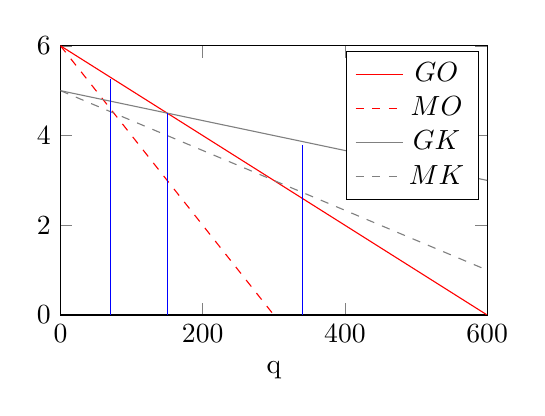
\begin{tikzpicture}
	\begin{axis}[name=left,xlabel={q}, ylabel={}, ymin=0,ymax=6,xmin=0,xmax=600,width=7cm, height=5cm]
		\addplot[red, samples=50, domain=0:600]{6-(1/100)*x};
		\addplot[red,dashed,samples=50, domain=0:600]{6-(2/100)*x};
		\addplot[gray,samples=50, domain=0:600]{5-(1/300)*x};
		\addplot[gray,dashed,samples=50, domain=0:600]{5-(1/150)*x};
		\addplot[blue] coordinates {(70,0) (70,5.25)};
		\addplot[blue] coordinates {(150,0) (150,4.5)};
		\addplot[blue] coordinates {(340,0) (340,3.8)};
		\legend{$GO$,$MO$,$GK$,$MK$}
	\end{axis}
\end{tikzpicture}
\caption{Kosten- \& opbrengstfuncties bij een natuurlijk monopolie (de verticale blauwe lijnen geven prijskeuzes weer - m\'et of zonder overheidsinterventie)}
\label{fig:h3natmon2}
\end{figure}

Wat is het beleid bij natuurlijke monopolies? Figuur \ref{fig:h3natmon2} geeft een voorbeeld van kost- \& opbrengstfuncties in dergelijke context. Wordt de monopolist vrijgelaten, dan zal hij zeer weinig verkopen tegen zeer hoge prijs (linkse blauwe lijn).
\par Past men \textit{marginal cost pricing} toe, dan zal de prijs gelijk gesteld worden aan de marginale kost (rechtse blauwe lijn). Dit zou echter verlies veroorzaken (de gemiddelde opbrengst is lager dan de gemiddelde kost). Dus gaat men een gulden middenweg kiezen (blauwe lijn in het midden).\\

\par In de context van deze welvaartsanalyse kan men ook even het begrip \entrystyled{statische efficientie}{statische effici\"entie} en het begrip \entrystyled{dynamische efficientie}{dynamische effici\"entie} bespreken.
\par Het eerste gaat over het optimaal aanwenden van de \textit{bestaande} productiemiddelen. Dit gaat over \entrystyled{pareto-efficientie}{Pareto-effici\"entie} en dus niet over verdeling.
\par Het tweede gaat over hoe men de optimale uitbreiding van de productiecapaciteit in de hand werkt. Dit gaat over lange termijn economische groei.\\

\par Monopolies zijn statisch ineffici\"ent en mogelijks dynamisch effici\"ent. Zo kan een tijdelijk monopolie (een \entry{patent} of \entry{octrooi}) een prikkel zijn om innovatie tot stand te brengen. Dat zorgt voor meer uitvindingen die echter slechter gebruikt worden. Men zoekt naar de optimale duur voor een patent om hier een evenwicht in te vinden.
\par Daarnaast kan tolerantie tegenover monopolies (men laat ze winst maken) leiden tot een relatief hoge winst die als bron van \term{autofinanciering} kan fungeren. Een deel van de winst wordt ge\"investeerd in het bedrijf zelve. Dergelijke autofinanciering is een aangepaste vorm van investeringen in onderzoek ; als je bijvoorbeeld investeert in antibiotica, dan is het perfect mogelijk dat dit mislukt. Dergelijke risicovolle investeringen zullen banken gewoonlijk niet willen financieren. Autofinanciering biedt een alternatief.

\subsection{Onvolmaakte Mededinging}

Naast de voorgaande heb je een aantal andere (realistischere) marktvormen (zie tabel \ref{tab:h3vormen}) ; het homogeen oligopolie, het heterogeen oligopolie en de monopolistische mededinging. Wij gaan deze nu bespreken.
\par Herinner dat we ervan uit gaan dat er veel vragers zijn en dat de agenten perfect ge\"informeerd zijn.

\subsubsection{Homogeen Oligopolie}

Het \entry{homogeen oligopolie} is een \entry{oligopolie} met weinig aanbieders van een homogeen product. Wij nemen een \entry{duopolie} als voorbeeld.\\

\par Stel, we hebben twee producenten die goed overeenkomen, en dan een \entry{kartel} vormen. Hun doel is dus de gezamenlijke winst te maximaliseren.
\par Om de zaken eenvoudig te houden werken we met een constante gemiddelde kost gelijk aan $2$. Als marktvraag (naar broodjes) nemen we $q=600-100p$. De inverse marktvraag is dan $p=6-0.01q$. De totale ontvangstenfunctie is $TO=pq=6q-0.01q^2$. En de marginale ontvangstencurve is $MO=6-0.02q$.\\

\par In dit voorbeeld is de optimale geproduceerde hoeveelheid (bij $MO=6-0.02q=2=MK$) gelijk aan $q=200$. Omdat we te maken hebben met twee aanbieders zal iedere aanbieder 100 producten produceren. De prijs is gelijk aan 4, de totale winst is 400 (200 per aanbieder).\\

\paragraph{De Prikkel om een Afspraak te Breken}

Helaas ... het duopolie loopt niet zo maar van een leien dakje. Beide aanbieders voelen de drang om hun afspraak te breken. Stel dat de eerste aanbieder (aanbieder $A$) dat doet. De inverse vraagcurve wordt $p=0.01(q_A+100)=5-0.01q_A$ (de tweede aanbieder produceert 100 producten omdat die de overeenkomst respecteert). De totale ontvangst wordt $TO_A=5q_A-0.01q_A^2$, de marginale ontvangst wordt $MO_A=5-0.02q_A$, en de optimale hoeveelheid wordt $q_A=150$. 
\par De aanbieder breidt zijn productie dus uit. Hierdoor wordt de prijs 3.5, waardoor de winst van $A$ ($TW_A=(3,5-2)*150=225$) \textit{verhoogt} en de winst van $B$ ($TW_B=(3.5-2)*100=150$) \textit{verlaagt} (zie figuur \ref{fig:h3duopolie}). De bedrieger heeft 25 winst meer, en de bedrogene verliest 50. De gezamenlijke winst is dus verlaagd. En dus zal de tweede aanbieder reageren ...

\begin{figure}[H]
\vspace{0.5cm}
\centering
\captionsetup{justification=centering,margin=2cm}
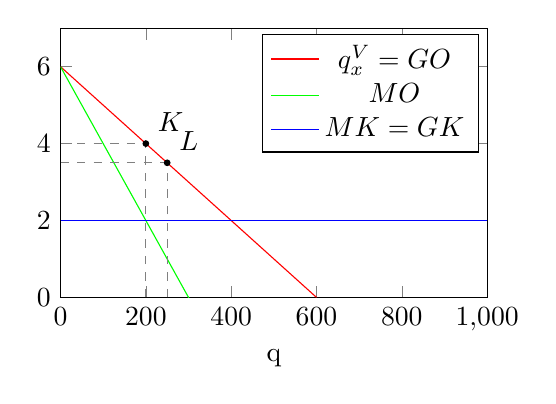
\begin{tikzpicture}
	\begin{axis}[name=left,xlabel={q}, ymin=0,ymax=7,xmin=0,xmax=1000,width=7cm, height=5cm]
		\addplot[red, samples=100, domain=0:600]{6-0.01*x};
		\addplot[green, samples=100, domain=0:600]{6-0.02*x};
		\addplot[blue, samples=100, domain=0:1000]{2};
		\addplot[gray,dashed] coordinates {(0,4) (200,4)};
		\addplot[gray,dashed] coordinates {(0,3.5) (250,3.5)};
		\addplot[gray,dashed] coordinates {(200,0) (200,4)};
		\addplot[gray,dashed] coordinates {(250,0) (250,3.5)};
		\node[label=above right:{$K$},minimum size=2pt, fill=black, inner sep=0pt, shape=circle, draw] at (axis cs:200, 4) {};
		\node[label=above right:{$L$},minimum size=2pt, fill=black, inner sep=0pt, shape=circle, draw] at (axis cs:250, 3.5) {};
		% \addplot+[draw=none,mark=none,pattern=flexible hatch, samples=100, domain=0:100, area legend, pattern color=gray!20]{100-(x*x)/100} \closedcycle;
		\legend{$q_x^V=GO$,$MO$,$MK=GK$}
	\end{axis}
\end{tikzpicture}
\caption{Het gegeven duopolie bij een karteloplossing ($K$) en bij een gebroken afspraak ($L$)}
\label{fig:h3duopolie}
\end{figure}

\paragraph{De Reactiefunctie en het Cournot-Evenwicht}

Stel dat de eerste aanbieder, aanbieder $A$ de overeenkomst met $B$ niet respecteert, maar er deze keer van uit gaat dat $B$ hetzelfde doet. Dan is de inverse vraagfunctie voor $A$ gelijk aan $p=6-0.01(q_A+q_B)$. Deze keer gaat $A$ er dus \textit{niet} van uit dat $q_B=100$ zoals dat in de karteloplossing het geval was.
\par De totale ontvangst is dan $TO_A=pq_A=6q_A-0.01q_A^2-0.01q_Aq_B$, de marginale ontvangst $MO_A=6-0.02q_A-0.01q_B$. De hoeveelheid die $A$ moet produceren om zijn winst te maximaliseren (bij $MO_A=MK$) is $q_A=200-0.5q_B$.\\

\par Men kan dezelfde redenering uiteraard toepassen voor $B$. Diens winstmaximaliserende output is dan hetzelfde, namelijk $q_B=200-0.5q_A$.
\par Dit zorgt voor een situatie waar $A$ reageert op $B$ en $B$ reageert op $A$, wat grafisch wordt voorgesteld in figuur \ref{fig:h3duopolie2}.

\begin{figure}[H]
\vspace{0.5cm}
\centering
\captionsetup{justification=centering,margin=2cm}
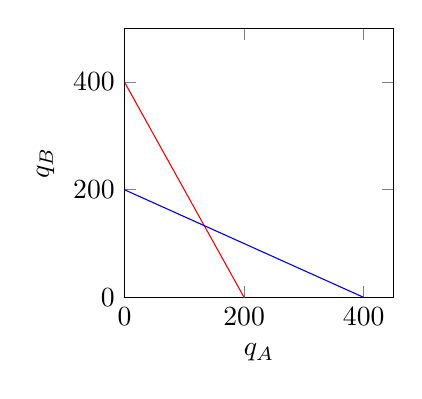
\begin{tikzpicture}
	\begin{axis}[name=left,xlabel={$q_A$},ylabel={$q_B$}, ymin=0,ymax=500,xmin=0,xmax=450,width=5cm, height=5cm]
		\addplot[red, samples=100, domain=0:400]{400-2*x};
		\addplot[blue, samples=100, domain=0:400]{200-0.5*x};
	\end{axis}
\end{tikzpicture}
\caption{Winstmaximaliserende output bij gegeven productiehoeveelheid van de andere aanbieder in het gegeven duopolie}
\label{fig:h3duopolie2}
\end{figure}

Een evenwicht wordt bereikt wanneer de twee curven in de figuur snijden. Dit noemt men een \entrystyled{cournot-evenwicht}{Cournot-evenwicht}. Algebra\"isch betekent dit dat $q_A=200-0.5q_B=200-0.5(200-0.5q_A)=100+0.25\Rightarrow q_A=\frac{100}{0.75}\approx 133$. Het marktaanbod is ongeveer 266 (broodjes), want $A$ en $B$ produceren evenveel.
\par De prijs is $p\approx 6-0.01*266\approx 3.34$. De totale winst per onderneming is $133*(3.34-2)\approx178.22$, en is dus \textit{kleiner} dan bij de karteloplossing.
\par Het Cournot-evenwicht wordt ook weergegeven in figuur \ref{fig:h3duopolie3}.

\begin{figure}[H]
\vspace{0.5cm}
\centering
\captionsetup{justification=centering,margin=2cm}
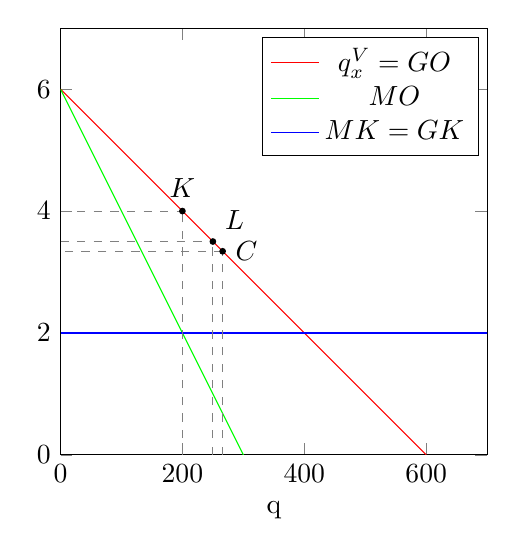
\begin{tikzpicture}
	\begin{axis}[name=left,xlabel={q}, ymin=0,ymax=7,xmin=0,xmax=700,width=7cm, height=7cm]
		\addplot[red, samples=100, domain=0:600]{6-0.01*x};
		\addplot[green, samples=100, domain=0:600]{6-0.02*x};
		\addplot[blue, samples=100, domain=0:1000]{2};
		\addplot[gray,dashed] coordinates {(0,4) (200,4)};
		\addplot[gray,dashed] coordinates {(0,3.5) (250,3.5)};
		\addplot[gray,dashed] coordinates {(200,0) (200,4)};
		\addplot[gray,dashed] coordinates {(250,0) (250,3.5)};
		\addplot[gray,dashed] coordinates {(266,0) (266,3.34)};
		\addplot[gray,dashed] coordinates {(266,3.34) (0,3.34)};
		\node[label=above:{$K$},minimum size=2pt, fill=black, inner sep=0pt, shape=circle, draw] at (axis cs:200, 4) {};
		\node[label=above right:{$L$},minimum size=2pt, fill=black, inner sep=0pt, shape=circle, draw] at (axis cs:250, 3.5) {};
		\node[label=right:{$C$},minimum size=2pt, fill=black, inner sep=0pt, shape=circle, draw] at (axis cs:266, 3.34) {};
		% \addplot+[draw=none,mark=none,pattern=flexible hatch, samples=100, domain=0:100, area legend, pattern color=gray!20]{100-(x*x)/100} \closedcycle;
		\legend{$q_x^V=GO$,$MO$,$MK=GK$}
	\end{axis}
\end{tikzpicture}
\caption{Het gegeven duopolie bij een karteloplossing ($K$), bij gebroken afspraak ($L$) en bij een Cournot-evenwicht ($C$)}
\label{fig:h3duopolie3}
\end{figure}

Dit hele verhaal kan men herformuleren aan de hand van de \entry{speltheorie}. Het oligopolie is immers een marktvorm met strategische interactie ; wat de ene doet hangt af van wat hij denkt dat de andere doet. De agenten spelen dus een spel ...

\subsubsection{Het Homogeen Oligopolie en Speltheorie}

We nemen even een voorbeeld van een spel. Stel, we hebben twee spelers ; $K$ en $R$. Elke speler heeft meerdere strategie\"en (ze kunnen elk kiezen tussen twee opties). Aan elke keuze is een resultaat verbonden. Dit wordt weergegeven in de resultatenmatrix in tabel \ref{tab:h3spel}.

\begin{table}[H]
\small\centering\captionsetup{justification=centering,margin=2cm}
\begin{tabular}{
>{\columncolor[HTML]{EFEFEF}}l |lll}
\cline{2-4}
\cellcolor[HTML]{FFFFFF}{\color[HTML]{FFFFFF} } & \multicolumn{3}{c|}{\cellcolor[HTML]{EFEFEF}$K$} \\ \hline
\multicolumn{1}{|l|}{\cellcolor[HTML]{EFEFEF}} &  & $T_1$ & $T_2$ \\
\multicolumn{1}{|l|}{\cellcolor[HTML]{EFEFEF}} & $S_1$ & A;B & C;D \\
\multicolumn{1}{|l|}{\multirow{-3}{*}{\cellcolor[HTML]{EFEFEF}$R$}} & $S_2$ & E;F & G;H \\ \cline{1-1}
\end{tabular}
\caption{Algemene resultatenmatrix (als $K$ keuze $T_1$ maakt en $R$ keuze $S_1$, dan is $A$ het resultaat voor $K$ en $B$ het resultaat voor $R$)}
\label{tab:h3spel}
\end{table}

\par\noindent Men spreekt van een \entry{dominante strategie} als het over een keuze gaat die \textit{hoe dan ook} de beste is. 
\par Stel dat $S_1$ zo'n dominante strategie is (en $S_2$ dus een \entry{gedomineerde strategie} is), dan houdt dit voor onze algemene resultatenmatrix in dat $A>E$ en $C>G$.
\par Is $T_1$ een dominante strategie, dan betekent dit dat $B>D$ en $F>H$.\\

\par\noindent Men spreekt van een \entrystyled{nash-evenwicht}{Nash-evenwicht} als een combinatie strategie\"en ertoe leidt dat geen van de spelers er baat bij heeft zijn strategie te veranderen. $(S_1,T_1)$ is dus een Nash-evenwicht als $A>E$ \'en $B>D$.
\par Een Nash-evenwicht is eigenlijk een minder strengere vorm van een evenwicht in dominante strategie\"en ; \textit{niet} elk Nash-evenwicht is een evenwicht in dominante strategie\"en, maar elk evenwicht in dominante strategie\"en is \textit{wel} een Nash-evenwicht.\\

\par\noindent Laten we nu een minder algemeen voorbeeld nemen\footnote{Het bekende en vaak gebruikte \textit{prisoner dilemma}.}.
\par Twee kompanen plegen een bankoverval, maar worden later aangehouden. Men ontdekt dat ze wapens bij zich hebben. Ze worden minstens veroordeeld voor illegaal wapenbezit, maar of ze worden veroordeeld voor de bankoverval hangt af van of ze bekennen. 
\par Dit wisten de twee kompanen niet op voorhand. Zij willen nu zo weinig mogelijk tijd in de gevangenis doorbrengen, wat wordt bepaald door de keuze die elk van hen maakt - bekennen of ontkennen (zie tabel \ref{tab:h3spel2}).

\begin{table}[H]
\small\centering\captionsetup{justification=centering,margin=2cm}
\begin{tabular}{
>{\columncolor[HTML]{EFEFEF}}l |lll}
\cline{2-4}
\cellcolor[HTML]{FFFFFF}{\color[HTML]{FFFFFF} } & \multicolumn{3}{c|}{\cellcolor[HTML]{EFEFEF}Gevangene 2} \\ \hline
\multicolumn{1}{|l|}{\cellcolor[HTML]{EFEFEF}} &  & $T_1$:bekennen & $T_2$:ontkennen \\
\multicolumn{1}{|l|}{\cellcolor[HTML]{EFEFEF}} & $S_1$:bekennen & (8 jaar, 8 jaar) & (1 jaar, 10 jaar) \\
\multicolumn{1}{|l|}{\multirow{-3}{*}{\cellcolor[HTML]{EFEFEF}Gevangene 1}} & $S_2$:ontkennen & (10 jaar, 1 jaar) & (2 jaar, 2 jaar) \\ \cline{1-1}
\end{tabular}
\caption{De resultatenmatrix voor het gevangenendilemma}
\label{tab:h3spel2}
\end{table}

In dit dilemma is bekennen telkens een dominante strategie, en ontkennen een gedomineerde strategie. En dat illustreert hoe, als iedereen zijn eigenbelang nastreeft (er is geen co\"operatie), het gezamenlijk belang niet noodzakelijk wordt behartigd.  Bij volmaakte mededinging is dat wel zo, maar bij onvolmaakte mededinging niet.

\par\noindent We nemen nog een ander (vereenvoudigd) voorbeeld. Stel, we hebben een fietser en een automobilist. Als de fietser voorzorg neemt, dan kost dat hem 20. Als de autobestuurder dat doet, kost dat hem 30. 
\par Is er een botsing, dan kost de schade 60 indien zowel fietser als automobilist voorzorg hebben genomen. Als de fietser geen en de automobilist wel voorzorg heeft genomen, dan kost de schade 100. Als de fietser wel en automobilist geen voorzorg heeft genomen, dan kost de schade 120. Hebben geen van beiden voorzorg genomen, dan kost de schade 150. We gaan ervan uit dat de automobilist aansprakelijk is voor de schade als de fietser voorzorg heeft genomen.
\par De resultatenmatrix zie je in tabel \ref{tab:h3spel3}.

\begin{table}[H]
\small\centering\captionsetup{justification=centering,margin=2cm}
\begin{tabular}{l|lll}
\cline{2-4}
 & \multicolumn{3}{c|}{\cellcolor[HTML]{EFEFEF}Automobilist} \\ \hline
\multicolumn{1}{|l|}{\cellcolor[HTML]{EFEFEF}} &  & NV & GV \\
\multicolumn{1}{|l|}{\cellcolor[HTML]{EFEFEF}} & NV & 20;90 & 20;120 \\
\multicolumn{1}{|l|}{\multirow{-3}{*}{\cellcolor[HTML]{EFEFEF}Fietser}} & GV & 100;30 & 150;0 \\ \cline{1-1}
\end{tabular}
\caption{De resultatenmatrix voor het fietser- en automobilist probleem (NV = noodzakelijke voorzorg, GV = geen voorzorg)}
\label{tab:h3spel3}
\end{table}

Voor de fietser is de dominante strategie de noodzakelijke voorzorg (NV). Als de fietser hiervoor kiest, is enkel de eerste rij relevant voor de automobilist, en is NV ook voor hem een dominante strategie. De combinatie van beide keuzes levert een Nash-evenwicht, maar geen evenwicht in dominante strategie\"en. Het is tevens ook een \textit{uniek} Nash-evenwicht.\\

\par In tabel \ref{tab:h3spel4} is een voorbeeldspel met twee Nash-evenwichten. Het gaat over een koppel dat moet beslissen of ze naar een voetbalmatch gaan kijken of naar de bioscoop gaan.

\begin{table}[H]
\small\centering\captionsetup{justification=centering,margin=2cm}
\begin{tabular}{l|lll}
\cline{2-4}
 & \multicolumn{3}{c|}{\cellcolor[HTML]{EFEFEF}Strategie\"en voor mevrouw} \\ \hline
\multicolumn{1}{|l|}{\cellcolor[HTML]{EFEFEF}} &  & $t_1$:voetbal & $t_2$:bioscoop \\
\multicolumn{1}{|l|}{\cellcolor[HTML]{EFEFEF}} & $s_1$:voetbal & 3;1 & 0;0 \\
\multicolumn{1}{|l|}{\multirow{-3}{*}{\cellcolor[HTML]{EFEFEF}Strategie\"en voor meneer}} & $s_2$:bioscoop & 0;0 & 1;3 \\ \cline{1-1}
\end{tabular}
\caption{De resultatenmatrix voor het \textit{`battle of the sexes'} probleem (de man heeft een voorkeur voor voetbal, en de vrouw heeft een voorkeur voor de bioscoop, maar ze willen niet alleen gaan}
\label{tab:h3spel4}
\end{table}

Zowel $(s_1,t_1)$ als $(s_2,t_2)$ zijn Nash-evenwichten. Welke keuze wordt gemaakt hangt af van de machtspositie van beide.\\

\par De voorgaande spellen waren vereenvoudigde voorbeelden om de concepten uit te leggen. Men kan dit nu gebruiken voor het homogeen duopolie dat men voorheen besprak. De (ietwat complexere) resultatenmatrix vind je in tabel \ref{tab:h3resduo}.

\begin{table}[H]
\small\centering\captionsetup{justification=centering,margin=2cm}
\begin{tabular}{c|
>{\columncolor[HTML]{F9F9F9}}l llll}
\cline{2-6}
\multicolumn{1}{l|}{} & \multicolumn{5}{c|}{\cellcolor[HTML]{EFEFEF}Strategie\"en voor duopolist B} \\ \hline
\multicolumn{1}{|c|}{\cellcolor[HTML]{EFEFEF}} &  & \cellcolor[HTML]{F9F9F9}$t_1:q_B=50$ & \cellcolor[HTML]{F9F9F9}$t_2:q_B=100$ & \cellcolor[HTML]{F9F9F9}$t_3:q_B=133$ & \cellcolor[HTML]{F9F9F9}$t_4:q_B=150$ \\
\multicolumn{1}{|c|}{\cellcolor[HTML]{EFEFEF}} & $s_1:q_A=50$ & (150;150) & (125;250) & (109;289) & (100;300) \\
\multicolumn{1}{|c|}{\cellcolor[HTML]{EFEFEF}} & $s_2:q_A=100$ & (250;125) & \begin{tabular}[c]{@{}l@{}}(200;200)\\ \textit{karteluitkomst}\end{tabular} & (167;222) & (150;225) \\
\multicolumn{1}{|c|}{\cellcolor[HTML]{EFEFEF}} & $s_3:q_A=133$ & (289;109) & (222;167) & \begin{tabular}[c]{@{}l@{}}(178;178)\\ \textit{Nash-evenwicht}\end{tabular} & (156;176) \\
\multicolumn{1}{|c|}{\multirow{-5}{*}{\cellcolor[HTML]{EFEFEF}Strategie\"en voor duopolist A}} & $s_4:q_A=150$ & (300;100) & (225;150) & (176;156) & (150;150) \\ \cline{1-1}
\end{tabular}
\caption{De resultatenmatrix voor het \textit{`battle of the sexes'} probleem (de man heeft een voorkeur voor voetbal, en de vrouw heeft een voorkeur voor de bioscoop, maar ze willen niet alleen gaan}
\label{tab:h3resduo}
\end{table}

Eerst is er de karteloplossing. Maar deze is geen evenwicht, gezien beide partijen er baat bij hebben om van gedachte te veranderen. Daarom breekt duopolist $A$ de afspraak en produceert hij $q_A=150$, waarna $B$ zich aanpast en $q_B\approx 133$ produceert, waarna $A$ zich daaraan aanpast en $q_A\approx 133$ produceert. En dan heb je een Nash-evenwicht!
\par Merk op dat we dit eerder het \entrystyled{cournot-evenwicht}{Cournot-evenwicht} noemden. Het Cournot-evenwicht is een voorbeeld van een Nash-evenwicht, maar het Nash-evenwicht is een breder concept. Merk op dat het Nash-evenwicht hier \textit{geen} evenwicht in dominante strategie\"en is.

\paragraph{De Paradox van Bertrand}

Cournot, die het Cournot-evenwicht bedacht, werd bekritiseerd door een andere Fransman, met name meneer Bertrand.
\par Bertrand merkte op dat, voor Cournot, de beslissingsvariabele de \textit{hoeveelheid} is. Hij stelde voor om in de plaats hiervan met de prijs te werken. De concurrentie gebeurt dus via prijs, niet via hoeveelheid.\\

\par In ons voorbeeld-duopolie was de prijs ongeveer $3,34$. Beide aanbieders zullen graag hun prijs verlagen (niet verhogen, want de producten zijn homogeen, dus zouden de klanten in dat geval gewoon verdwijnen). 
\par Een lage prijs zetten is dus de dominante strategie, het is de beste strategie ongeacht het gedrag van de consument. Dit leidt er uiteindelijk toe dat beide ondernemingen hun prijs laten dalen tot de prijs gelijk is aan het minimum van de gemiddelde kosten. Net zoals bij volmaakte mededinging is dit ideaal voor de consumenten.
\par En dus kan men besluiten dat indien ondernemingen in een homogeen duopolie elkaar beconcurreren, dat men paradoxalerwijze dezelfde uitkomst krijgt als bij perfecte mededinging (het consumentensurplus is maximaal, er is \entrystyled{pareto-efficientie}{Pareto-effici\"entie}).

\subsubsection{Productdifferentiatie}

Bertrand werd op zijn beurt bekritiseerd door een zekere Hotelling. Deze had het specifiek over \entry{productdifferentiatie}. Dat betekent dat producten van elkaar verschillen waardoor aanbieders bepaalde vragers kunnen aantrekken (dit kan via reclame, wat uiteindelijk neerkomt op liegen).

\paragraph{Het Hotelling Model bij een Oligopolie}

Stel, men heeft twee ijsverkopers aan de kust. Het strand is twee kilometer lang, en elke verkoper bevindt zich op 500 meter van het linker- respectievelijk rechter-uiteinde (figuur \ref{fig:h3strand}). Stel dan ook dat er een aantal toeristen zijn die zin hebben in ijs. Als ze het niet erg vinden om ver te moeten stappen (er is afwezigheid van verplaatsingskosten), dan zijn de producten (het ijs) homogeen. Dan gaan ze enkel naar de prijs kijken en eindigt men met het Bertrand-evenwicht. \\

\begin{figure}[H]
\vspace{0.5cm}
\centering
\captionsetup{justification=centering,margin=2cm}
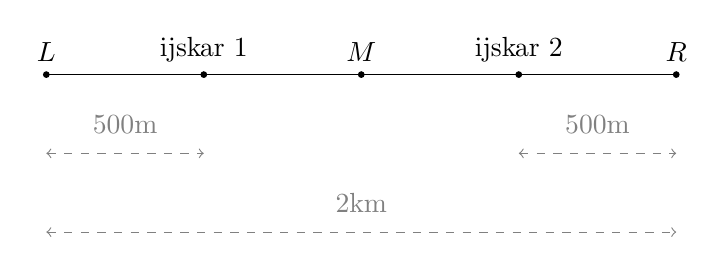
\begin{tikzpicture}
\draw (0,2) -- (8,2);
\node[label=above:{$L$},minimum size=2pt, fill=black, inner sep=0pt, shape=circle, draw] at (0,2) {};
\node[label=above:{$R$},minimum size=2pt, fill=black, inner sep=0pt, shape=circle, draw] at (8,2) {};
\node[label=above:{$M$},minimum size=2pt, fill=black, inner sep=0pt, shape=circle, draw] at (4,2) {};
\node[label=above:{ijskar 1},minimum size=2pt, fill=black, inner sep=0pt, shape=circle, draw] at (2,2) {};
\node[label=above:{ijskar 2},minimum size=2pt, fill=black, inner sep=0pt, shape=circle, draw] at (6,2) {};
\draw[<->,gray, dashed] (0,1) -- (1,1) node [label=above:{500m}] {} -- (2,1);
\draw[<->,gray, dashed] (6,1) -- (7,1) node [label=above:{500m}] {} -- (8,1);
\draw[<->,gray, dashed] (0,0) -- (4,0) node [label=above:{2km}] {} -- (8,0);
\end{tikzpicture}
\caption{Twee ijsverkopers aan het strand}
\label{fig:h3strand}
\end{figure}

\par Als de toeristen het \textit{niet} leuk vinden om ver te moeten stappen, dan zijn er w\'el verplaatsingskosten. Dat betekent dat er 
\entry{productdifferentiatie} is. Beide ijsverkopers hebben \entry{marktmacht} ; elke venter heeft zijn eigen cli\"enteel (een \entry{niche}) waarmee hij winst kan realiseren. Het zijn de toeristen die dichterbij staan. Het Bertrand-evenwicht zal dus niet meer opgaan, want elke verkoper kan zijn prijs aanpassen zonder dat het de andere verkoper be\"invloedt.\\

\par Hoewel er echter geen prijsconcurrentie is, is differentiatiebeleid wel mogelijk. Om meer klanten te hebben zal elke ijsverkoper zijn kar naar het midden van het strand verplaatsen. Wanneer ze dat beiden doen, dan zijn hun producten alsnog homogeen, is er weer prijscompetitie, en eindigt men weer met een Bertrand-evenwicht.\\

\par Onder bepaalde voorwaarden zal men \textit{extreme} differentiatie krijgen. Als de ijskarren zich aan de uiteinden vinden van het strand, bijvoorbeeld. Dat is een suboptimaal evenwicht. Het optimaal evenwicht is de eerste situatie ; beide bevinden zich op 500 meter van de uiteinden van het strand.

\paragraph{Monopolistische Mededinging}

Productdifferentiatie komt ook voor bij de \entry{monopolistische mededinging}. Dat is een marktvorm waarbij iedere aanbieder een eigen niche heeft. De ondernemingsvraag heeft dan betrekking op zijn variant van het goed, en is daarom niet perfect elastisch.
\par De marktvorm vertoont echter ook kenmerken van volmaakte mededinging. Er zijn immers veel aanbieders door vrije toe- en uittreding, er zijn veel vragers die van vele aanbieders kopen, en wat de ene aanbieder doet, dat voelen de anderen niet veel. De producenten doen niet aan strategische interactie. Speltheorie is dus niet toepasselijk\footnote{De speltheorie is typisch voor het oligopolie, maar is niet toepasselijk bij de volmaakte mededinging, het monopolie en de monopolistische mededinging.}.

\begin{figure}[H]
\vspace{0.5cm}
\centering
\captionsetup{justification=centering,margin=2cm}
\begin{tikzpicture}
	\begin{axis}[name=left,xlabel={q}, ylabel={$p$},ymin=12,ymax=21,xmin=0,xmax=35,width=7cm, height=7cm,yticklabels={,,},xticklabels={,,}]
		\addplot[red, samples=12, domain=0:35]{0.025*x^2-0.6*x+18.6};
		\addplot[gray, samples=50, domain=0:35]{0.075*x^2-1.2*x+18.6};
		\addplot[black, samples=50, domain=0:35]{18-0.25*x};
		\addplot[gray, dashed, samples=50, domain=0:35]{18-0.55*x};
		\node[label=below left:{$E$},minimum size=2pt, fill=black, inner sep=0pt, shape=circle, draw] at (axis cs:8, 13.8) {};
		\node[label=below left:{},minimum size=2pt, fill=black, inner sep=0pt, shape=circle, draw] at (axis cs:8,16) {};
		\node[label=below left:{},minimum size=2pt, fill=black, inner sep=0pt, shape=circle, draw] at (axis cs:8,15.4) {};
		\addplot[blue,dashed] coordinates {(8,0) (8,16)};
		\addplot[blue,dashed] coordinates {(8,16) (0,16)};
		\addplot[blue,dashed] coordinates {(8,15.4) (0,15.4)};
		\addplot[draw=none,pattern=north west lines, pattern color=gray!20] coordinates {(0,16) (8,16) (8,15.4) (0,15.4)};
		\legend{$GK$, $MK$,$V=GO$,$MO$}
	\end{axis}
\end{tikzpicture}
\caption{Het evenwicht bij een monopolistische mededinging op korte termijn (de winst is gearceerd)}
\label{fig:h3monmed}
\end{figure}

In den beginne gaat er bij monopolistische mededinging een evenwicht zijn zoals bij het monopolie ($MO=MK$, zie figuur \ref{fig:h3monmed}).\\

\par Als een producent veel winst maakt zullen er producenten bijkomen en zal de vraag vergroten. Daardoor moet men de vraag horizontaal optellen, en verplaatst de vraagfunctie naar links en wordt ie vlakker, tot de functie raakt aan de gemiddelde kost (zie figuur \ref{fig:h3monmed2}).

\begin{figure}[H]
\vspace{0.5cm}
\centering
\captionsetup{justification=centering,margin=2cm}
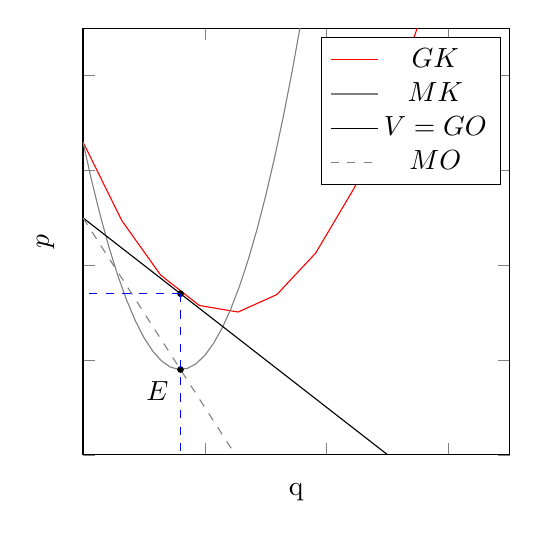
\begin{tikzpicture}
	\begin{axis}[name=left,xlabel={q}, ylabel={$p$},ymin=12,ymax=21,xmin=0,xmax=35,width=7cm, height=7cm,yticklabels={,,},xticklabels={,,}]
		\addplot[red, samples=12, domain=0:35]{0.025*x^2-0.6*x+18.6};
		\addplot[gray, samples=50, domain=0:35]{0.075*x^2-1.2*x+18.6};
		\addplot[black, samples=50, domain=0:35]{17-0.2*x};
		\addplot[gray, dashed, samples=50, domain=0:35]{17-0.4*x};
		\node[label=below left:{$E$},minimum size=2pt, fill=black, inner sep=0pt, shape=circle, draw] at (axis cs:8, 13.8) {};
		\node[label=below left:{},minimum size=2pt, fill=black, inner sep=0pt, shape=circle, draw] at (axis cs:8,15.4) {};
		\addplot[blue,dashed] coordinates {(8,15.4) (0,15.4)};
		\addplot[blue,dashed] coordinates {(8,15.4) (8,0)};
		\legend{$GK$, $MK$,$V=GO$,$MO$}
	\end{axis}
\end{tikzpicture}
\caption{Het evenwicht bij een monopolistische mededinging op lange termijn (de winst is gearceerd)}
\label{fig:h3monmed}
\end{figure}

De winst is dus ge\"erodeerd door de concurrentie. En net zoals bij volmaakte mededinging is dat geen slechte zaak, want de producenten worden nog steeds betaald voor hun moeite.\\

\par Wat is dan het verschil met de volmaakte mededinging? Allereerst is de prijs hier niet gelijk aan de marginale kost, maar \textit{hoger}. Er is dus Pareto-ineffici\"entie.
\par Bovendien wordt er wel geproduceerd aan de gemiddelde kost, maar deze is hier \textit{niet} minimaal.
\par Het moet wel gezegd worden dat de producten bij volmaakte mededinging \textit{homogeen} zijn, dat wil zeggen, ze zijn allemaal hetzelfde. Mensen vinden het gewoonlijk fijner om uit een gamma te kunnen kiezen. Stel je voor dat alle auto's identiek zijn ... De voordelen van de volmaakte mededinging moeten dus genuanceerd worden. 

\subsubsection{Asymmetrische informatie}\label{sec:asyinfo}

We gingen tot nog toe uit van perfect ge\"informeerde agenten. In de werkelijkheid zijn er veel markten waar dat niet het geval is. Er is dan sprake van \entry{asymmetrische informatie}. Bij de verkoop van tweedehandswagens zijn de verkopers bijvoorbeeld beter ge\"informeerd dan de koper. Bij de markt voor autoverzekeringen is dat omgekeerd. \\

\par Door asymmetrische informatie gaan potentieel wederzijds voordelige transacties niet door. Om dit te illustreren gaan we even verder in op de markt voor tweedehandswagens. 
\par Stel, een verkoper vraagt 2100 euro's voor slechte wagens en 2700 euro's voor goede wagens. De koper wilt op zijn beurt respectievelijk 2400 euro's en 3000 euro's betalen.\\

\par De koper weet dat twee derde van alle wagens slecht is. Zijn betalingsbereidheid zakt hierdoor tot ($\frac{1}{3}\cdot 3000+\frac{2}{3}\cdot 2400=$) 2600 euro's. Hierdoor is er \entry{averechtse selectie} : de goede wagens verdwijnen uit de markt. Er is dus een \entry{missing market}. Dit kan verder gaan, waarbij de betere wagens steeds uit de markt verdwijnen tot de hele markt verdwenen is.
\par Dit fenomeen kan men oplossen via reputatie (een garage die gekend is voor zijn verkoop van goede wagens, bijvoorbeeld) en/of via controle.\\

\par We kijken nu naar het andere voorbeeld, de markt voor autoverzekeringen. In deze markt is het zo dat het individueel gedrag beter gekend is door de verzekeringnemer. Men heeft het over \entry{moral hazard}. De verzekeraar kent enkel het gemiddeld risico en bepaalt de premie in functie daarvan.
\par Hier kan er ook \entry{averechtse selectie} zijn als de goede risico's (die cli\"enten die het minst kans maken op auto-ongevallen) zich niet meer verzekeren. Want dan gaat de premie verhogen en zal de markt voor goede risico's verdwijnen. Dit kan uiteindelijk weer leiden tot het verdwijnen van de markt, wat kan opgelost worden met een verplichte verzekering, een bonus-malussysteem (de goede rijders worden beloond, de slechte rijders worden gestraft), of door andere premies uit te geven aan mensen van verschillende leeftijd en geslacht.
\par Er wordt af en toe een `zwarte doos' ge\"installeerd in een wagen om zo te bepalen hoe risicovol de autobestuurder is.\\


\subsubsection{Samenvatting}

De type marktvormen die we in dit hoofdstuk over onvolmaakte mededinging zagen zijn realistischer. Tabel \ref{tab:h3-kern} geeft een samenvattend overzicht.

\begin{table}[H]
\centering
\begin{tabular}{l|ll}
\cline{2-3}
 & \cellcolor[HTML]{EFEFEF}Homogeen & \multicolumn{1}{l|}{\cellcolor[HTML]{EFEFEF}Heterogeen} \\ \hline
\multicolumn{1}{|l|}{\cellcolor[HTML]{EFEFEF}Weinig aanbieders} & \begin{tabular}[c]{@{}l@{}}Cournot\\ Bertrand\\ Speltheorie\end{tabular} & \begin{tabular}[c]{@{}l@{}}Hotelling\\ Speltheorie\end{tabular} \\ \hline
\multicolumn{1}{|l|}{\cellcolor[HTML]{EFEFEF}Veel aanbieders} & \begin{tabular}[c]{@{}l@{}}Imperfecte informatie\\ Averechtse selectie\end{tabular} & Monopolistische concurrentie \\ \cline{1-1}
\end{tabular}
\caption{Een overzicht van de marktvormen van onvolmaakte mededinging}
\label{tab:h3-kern}
\end{table}

Meestal is de onvolmaaktheid in deze marktvormen een bron van Pareto-ineffici\"entie. Dan is er nood aan overheidsinterventie, om een Pareto-effici\"ente staat te bereiken\footnote{Dit is echter \textit{geen} Pareto-verbetering.}.\\

\par Dit geldt niet voor de volmaakte mededinging, het monopolie met perfecte prijsdiscriminatie en het Bertrand-evenwicht bij oligopolie. Deze zijn Pareto-effici\"ent. 








